\section{Lagrange Interpolation}
Use the method of Lagrange \textit{interpolation} to derive an expression for the mixed derivative, $u_{xy}$,  at the center of the stencil pictured below, i.e.  point (0,0), using the values of $u$ only at the four corner nodes in a uniform grid.  Note, this problem is solved using the method of undetermined coefficients in the notes.

\begin{figure}[h]
    \centering
    

\tikzset{every picture/.style={line width=0.75pt}} %set default line width to 0.75pt        

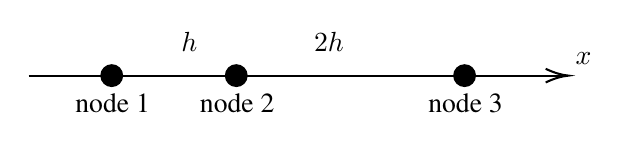
\begin{tikzpicture}[x=0.75pt,y=0.75pt,yscale=-1,xscale=1]
%uncomment if require: \path (0,300); %set diagram left start at 0, and has height of 300

%Straight Lines [id:da5299394466860707] 
\draw    (155,65) -- (413,65) ;
\draw [shift={(415,65)}, rotate = 180] [color={rgb, 255:red, 0; green, 0; blue, 0 }  ][line width=0.75]    (10.93,-3.29) .. controls (6.95,-1.4) and (3.31,-0.3) .. (0,0) .. controls (3.31,0.3) and (6.95,1.4) .. (10.93,3.29)   ;
%Shape: Circle [id:dp0275755717354893] 
\draw  [fill={rgb, 255:red, 0; green, 0; blue, 0 }  ,fill opacity=1 ] (190,65) .. controls (190,62.24) and (192.24,60) .. (195,60) .. controls (197.76,60) and (200,62.24) .. (200,65) .. controls (200,67.76) and (197.76,70) .. (195,70) .. controls (192.24,70) and (190,67.76) .. (190,65) -- cycle ;
%Shape: Circle [id:dp16091151773278578] 
\draw  [fill={rgb, 255:red, 0; green, 0; blue, 0 }  ,fill opacity=1 ] (250,65) .. controls (250,62.24) and (252.24,60) .. (255,60) .. controls (257.76,60) and (260,62.24) .. (260,65) .. controls (260,67.76) and (257.76,70) .. (255,70) .. controls (252.24,70) and (250,67.76) .. (250,65) -- cycle ;
%Shape: Circle [id:dp2533213412832751] 
\draw  [fill={rgb, 255:red, 0; green, 0; blue, 0 }  ,fill opacity=1 ] (360,65) .. controls (360,62.24) and (362.24,60) .. (365,60) .. controls (367.76,60) and (370,62.24) .. (370,65) .. controls (370,67.76) and (367.76,70) .. (365,70) .. controls (362.24,70) and (360,67.76) .. (360,65) -- cycle ;

% Text Node
\draw (227,42.4) node [anchor=north west][inner sep=0.75pt]    {$h$};
% Text Node
\draw (291,42.4) node [anchor=north west][inner sep=0.75pt]    {$2h$};
% Text Node
\draw (176,72) node [anchor=north west][inner sep=0.75pt]   [align=left] {{\fontfamily{ptm}\selectfont node 1}};
% Text Node
\draw (236,72) node [anchor=north west][inner sep=0.75pt]   [align=left] {{\fontfamily{ptm}\selectfont node 2}};
% Text Node
\draw (346,72) node [anchor=north west][inner sep=0.75pt]   [align=left] {{\fontfamily{ptm}\selectfont node 3}};
% Text Node
\draw (417,52.4) node [anchor=north west][inner sep=0.75pt]    {$x$};


\end{tikzpicture}

    \caption{Stencil for Lagrange interpolation.}
\end{figure}

\vspace{-0.35in}
\begin{align*}
    \shortintertext{To conduct the Lagrange interpolation, I will conduct evaluate at each node. Taking into consideration that this is in two-dimensions that the Lagrange interpolating functions can be expressed separetly to be}
    L_{-1}^z(z) & = \frac{(z - z_0)(z - z_{1})}{(-\Delta z)(-2 \Delta z)}, \quad \text{for node $j=-1$}\\
    L_{0}^z(z) & = \frac{(z - z_{-1})(z - z_{1})}{(\Delta z)(-\Delta z)}, \quad \text{for node $j=-0$}\\
    L_{1}^z(z) & = \frac{(z - z_{-1})(z - z_{0})}{(2\Delta z)(\Delta z)}, \quad \text{for node $j=1$}\\
    \shortintertext{Where $z$ is either $x,\ y$ depending on the node and evaluating at each of the nodes gives,}
\end{align*}

\vspace{-0.75in}
\begin{align*}
    N_{1,1} & = L_{1}(x)\ L_{1}(y)\\
        & = \left( \frac{(x - x_{-1})(x - x_{0})}{(2\Delta x)(\Delta x)} \right) \left( \frac{(y - y_{-1})(y - y_{0})}{(2\Delta y)(\Delta y)}  \right)\\
    N_{-1,-1} & = L_{-1}(x)\ L_{-1}(y)\\
        & = \left(\frac{(x - x_0)(x - x_{-1})}{(-\Delta x)(-2 \Delta x)}\right) \left( \frac{(y - y_0)(y - y_{-1})}{(-\Delta y)(-2 \Delta y)}\right)\\
    N_{1,-1} & = L_{1}(x)\ L_{-1}(y)\\
        & = \left( \frac{(x - x_{-1})(x - x_{0})}{(2\Delta x)(\Delta x)} \right) \left( \frac{(y - y_0)(y - y_{-1})}{(-\Delta y)(-2 \Delta y)}\right)\\
    N_{-1,1} & = L_{-1}(x)\ L_{1}(y)\\
        & = \left(\frac{(x - x_0)(x - x_{-1})}{(-\Delta x)(-2 \Delta x)}\right) \left( \frac{(y - y_{-1})(y - y_{0})}{(2\Delta y)(\Delta y)}  \right)
\end{align*}

\pagebreak
\pagestyle{fancy}
\restoregeometry

\begin{align*}
    \shortintertext{With all the Lagrange interpolating functions defined at each node the approximated solution can be expressed by the following relation,}
    \tilde{u} & = \sum_{j = -l}^{r}\sum_{k=-d}^{u}L_{j}^x(x)L_{k}^y(y)u_{k,j}\\
    \shortintertext{In order to evaluate the mixed derivative at the center point, each Nodal value must have its mixed derivative computed and evalued at $x_0,\ y_0$ so,}
    \frac{\partial ^2N_{1,1}}{\partial x\partial y}|_{x_0,\ y_0} & = \frac{(x_0 - 2x + x_{-1})(y_0 - 2y + y_{-1})}{4\Delta x^2\Delta y^2}|_{x_0,\ y_0}\\
    & = \frac{ \overbrace{(-x_0 + x_{-1})}^{-\Delta x} \overbrace{(-y_0 + y_{-1})}^{-\Delta y}}{4\Delta x^2 \Delta y^2}u_{1,1} = \frac{1}{4\Delta x\Delta y}u_{1,1}\\
    \frac{\partial ^2N_{-1,-1}}{\partial x\partial y}|_{x_0,\ y_0} & = \frac{(x_0 - 2x + x_{1})(y_0 - 2y + y_{1})}{4\Delta x^2\Delta y^2}|_{x_0,\ y_0}\\
    & = \frac{ \overbrace{(-x_0 + x_{1})}^{\Delta x} \overbrace{(-y_0 + y_{1})}^{\Delta y}}{4\Delta x^2 \Delta y^2}u_{-1,-1} = \frac{1}{4\Delta x\Delta y}u_{-1,-1}\\
    \frac{\partial ^2N_{1,-1}}{\partial x\partial y}|_{x_0,\ y_0} & = \frac{(x_0 - 2x + x_{-1})(y_0 - 2y + y_{1})}{4\Delta x^2\Delta y^2}|_{x_0,\ y_0}\\
    & = \frac{ \overbrace{(-x_0 + x_{-1})}^{-\Delta x} \overbrace{(-y_0 + y_{1})}^{\Delta y}}{4\Delta x^2 \Delta y^2}u_{1,-1} = -\frac{1}{4\Delta x\Delta y}u_{1,-1}\\
    \frac{\partial ^2N_{-1,1}}{\partial x\partial y}|_{x_0,\ y_0} & = \frac{(x_0 - 2x + x_{1})(y_0 - 2y + y_{-1})}{4\Delta x^2\Delta y^2}|_{x_0,\ y_0}\\
    & = \frac{ \overbrace{(-x_0 + x_{1})}^{\Delta x} \overbrace{(-y_0 + y_{-1})}^{-\Delta y}}{4\Delta x^2 \Delta y^2}u_{-1,1} = -\frac{1}{4\Delta x\Delta y}u_{-1,1}\\
    \shortintertext{Summing all the contributions and substituting back into the equation we get that,}
\end{align*}

\vspace{-0.2in}
\begin{equation*}
    \boxed{u_{xy} \approx \frac{1}{4\Delta x\Delta y}\left(u_{1,1} + u_{-1,-1} - \left(u_{1,-1} + u_{-1,1}\right)\right)}
\end{equation*}
